% document
\documentclass[10pt,graphics,aspectratio=169,table]{beamer}
\usepackage{../code}
\usepackage{csquotes}
\usepackage{hyperref}
\usepackage{tikz}
\usepackage{pgfplots}
% theme
\usetikzlibrary{arrows}
\tikzstyle{line}=[draw] % here
\usetikzlibrary{decorations.pathmorphing}
\tikzset{arrow/.style={-latex, shorten >=.5ex, shorten <=.5ex}}

\usetheme{metropolis}
% packages
\title{Lesson 4}
\author{Christian Schwarz, Jakob Krebs}
\date{18.11.2019}
\begin{document}
\maketitle

\begin{frame}{Contents}
    \tableofcontents
\end{frame}


\section{Source Code and Solutions}
\begin{frame}{Sources and Solutions}
    \begin{itemize}
        \item we publish all code written in this course at \url{https://github.com/jkrbs/c_lessons}
        \item we will publish example solutions of the tasks on same site
        \item send us questions or your solutions to c-lessons@deutschland.gmbh
    \end{itemize}
\end{frame}

\section{dynamic memory}
\begin{frame}[fragile]{A closer look at memory}
	\begin{tikzpicture}[y=2cm, font=\footnotesize]
		\node[above, font=\small] at (1.5,0) {Stack};
		
		\draw (0,0) -- (0,-2);
		\draw (0,0) -- (3,0);
		\draw (3,0) -- (3,-2);
		\draw[line join=round, decoration={zigzag,segment length=4, amplitude=1}, decorate] (0,-2) -- (3,-2);
		
		\draw[->] (-.25,0) -- (-.25,-1.9);
		
		\draw[dashed] (0,-.25) -- (3,-.25);
		\draw[dashed] (0,-.5) -- (3,-.5);
		\draw[dashed] (0,-.75) -- (3,-.75);
		\draw[dashed] (0,-1) -- (3,-1);
		\draw[dashed] (0,-1.25) -- (3,-1.25);
		\draw[dashed] (0,-1.5) -- (3,-1.5);
		\draw[dashed] (0,-1.75) -- (3,-1.75);
		
		\node[below, font=\small] at (6.5,-2) {Heap};		
		
		\draw (5,0) -- (5,-2);
		\draw[line join=round, decoration={zigzag,segment length=4, amplitude=1}, decorate] (5,0) -- (8,0);
		\draw (8,0) -- (8,-2);
		\draw (5,-2) -- (8,-2);
		
		\draw[<-] (8.25,-.1) -- (8.25,-2);
		
		\draw[dashed] (5,-.25) -- (8,-.25);
		\draw[dashed] (5,-.5) -- (8,-.5);
		\draw[dashed] (5,-.75) -- (8,-.75);
		\draw[dashed] (5,-1) -- (8,-1);
		\draw[dashed] (5,-1.25) -- (8,-1.25);
		\draw[dashed] (5,-1.5) -- (8,-1.5);
		\draw[dashed] (5,-1.75) -- (8,-1.75);
		
		\draw[thick, dashed, orange] (0,0) -- (3,0);
		\draw[thick, dashed, orange] (0,0) -- (0,-.25);
		\draw[thick, dashed, orange] (0,-.25) -- (3,-.25);
		\draw[thick, dashed, orange] (3,0) -- (3,-.25);
		\node[orange,below=.15em] at (1.5,0){int};

		\draw[thick, dashed, orange] (0,-.25) -- (3,-.25);
		\draw[thick, dashed, orange] (0,-.25) -- (0,-.5);
		\draw[thick, dashed, orange] (0,-.5) -- (3,-.5);
		\draw[thick, dashed, orange] (3,-.25) -- (3,-.5);
		\node[orange,below=.15em] at (1.5,-.25){int};
		
		\begin{uncoverenv}<3->
			\draw[thick, dashed, orange] (5,-1.75) -- (8,-1.75);
			\draw[thick, dashed, orange] (5,-1.75) -- (5,-2);
			\draw[thick, dashed, orange] (5,-2) -- (8,-2);
			\draw[thick, dashed, orange] (8,-1.75) -- (8,-2);
			\node[orange,below=.15em] at (6.5,-1.75){int};
		\end{uncoverenv}
		
		\begin{uncoverenv}<4->
			\draw[thick, dashed, teal] (0,-.5) -- (3,-.5);
			\draw[thick, dashed, teal] (0,-.5) -- (0,-1);
			\draw[thick, dashed, teal] (0,-1) -- (3,-1);
			\draw[thick, dashed, teal] (3,-.5) -- (3,-1);
			\node[teal,below=.15em] at (1.5,-.5){int*};
			
			\draw (3,-.75) edge[out=0,in=180,->,shorten >=.5ex, shorten <=.5ex] (5,-1.875);
		\end{uncoverenv}
		
		\begin{uncoverenv}<5->
			\draw[thick, dashed, purple] (5,-1.25) -- (8,-1.25);
			\draw[thick, dashed, purple] (5,-1.25) -- (5,-1.75);
			\draw[thick, dashed, purple] (5,-1.75) -- (8,-1.75);
			\draw[thick, dashed, purple] (8,-1.25) -- (8,-1.75);
			\node[purple, below=.15em] at (6.5,-1.25){long};
			
			\draw[thick, dashed, teal] (0,-1) -- (3,-1);
			\draw[thick, dashed, teal] (0,-1) -- (0,-1.5);
			\draw[thick, dashed, teal] (0,-1.5) -- (3,-1.5);
			\draw[thick, dashed, teal] (3,-1) -- (3,-1.5);
			\node[teal,below=.15em] at (1.5,-1){long*};
			
			\draw (3,-1.25) edge[out=0,in=180,->,shorten >=.5ex, shorten <=.5ex] (5,-1.5);
		\end{uncoverenv}
	\end{tikzpicture} \\
	\only<1>{All local variables of functions are placed at the \textit{stack}. \\
		It grows and shrinks as variables are declared and functions return.}
	\only<2>{Dynamical memory is allocated on the \textit{heap}. \\
		The example shows a function with two local \textit{int} variables.}
	\begin{onlyenv}<3>
		\begin{codeblock}[numbers=none]
malloc(sizeof(int));
\end{codeblock}
	Reserves exactly the amount of memory an \textit{int} variable takes.
	\end{onlyenv}
	\begin{onlyenv}<4>
		\begin{codeblock}[numbers=none]
int *new_block = malloc(sizeof(int));
\end{codeblock}
	The adress of that memory block is stored in an \textit{int} pointer.
	\end{onlyenv}
	\only<5>{\textit{malloc()} just needs to know the size of the block it reserves. \\
		Let us allocate a \textit{long} variable as well.}
\end{frame}


\begin{frame}[fragile]{\textit{malloc()} in detail}
	The function declaration might be a little bit confusing:
	\begin{codeblock}
void *malloc(size_t size);
    \end{codeblock}
	\begin{itemize}
		\item \textit{size} is the size of the reserved block in \textbf{bytes}. \\
		If you want to use that block \textit{seriously}, pass the size of an actual type (e.g. \textit{sizeof(int)}).
		\item A \textit{void} pointer is returned since \textit{malloc()} does not know how you want to use the reserved block. By assigning it to a regular pointer variable it is automatically converted to that type.
	\end{itemize}
\end{frame}
\begin{frame}[fragile]{Tidying up}
	Unlike normally declared variables, dynamically allocated storage is not automatically released when the function returns.
	\begin{codeblock}
void foo(void) {
	int *bar = malloc(sizeof *bar);
}
\end{codeblock}
	
With the pointer \textit{bar} being removed from the stack, we havo no reference on its allocated memory and those four bytes are blocked forever! \\
	\ \\
	\begin{codeblock}
free(void *ptr);
\end{codeblock}

Pass any pointer to previously allocated memory to \textit{free()} and it gets realeased.
\end{frame}

\section{Slightly Better User Input}

\begin{frame}[fragile]{The length of Strings}
    Last time we learned that we always need to pass the size of an array
    together with the pointer to it. So if strings are just \code{char} arrays,
    why do \code{puts} etc not require a size? 
  
    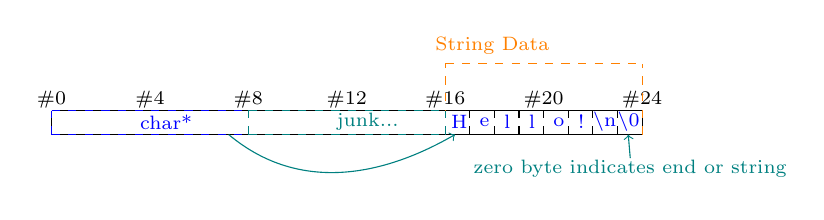
\begin{tikzpicture}[font=\scriptsize,x=2.5cm]
            
        \draw (0,1) -- (3,1);
        \draw (0,1) -- (0,1.3);
        \draw (0,1.3) -- (3,1.3);
        \draw (3,1) -- (3,1.3);

        \node[above=.6em] at (0,1) {\#0};
        \node[above=.6em] at (.5,1) {\#4};
        \draw[dashed] (1,1) -- (1,1.3);
        \node[above=.6em] at (1,1) {\#8};
        %\draw[dashed] (1.5,1) -- (1.5,1.3);
        \node[above=.6em] at (1.5,1) {\#12};
        \draw[dashed] (2.000,1) -- (2.000,1.3);
        \draw[dashed] (2.125,1) -- (2.125,1.3);
        \draw[dashed] (2.250,1) -- (2.250,1.3);
        \draw[dashed] (2.375,1) -- (2.375,1.3);
        \draw[dashed] (2.500,1) -- (2.500,1.3); 
        \draw[dashed] (2.625,1) -- (2.625,1.3);
        \draw[dashed] (2.750,1) -- (2.750,1.3);
        \draw[dashed] (2.875,1) -- (2.875,1.3); 
        \draw[dashed] (3.000,1) -- (3.000,1.3); 

        \node[blue, below=.4em, right=0em] at (1.980,1.3) {H};
        \node[blue, below=.4em, right=0em] at (2.125,1.3) {e};
        \node[blue, below=.4em, right=0em] at (2.250,1.3) {l};
        \node[blue, below=.4em, right=0em] at (2.375,1.3) {l};
        \node[blue, below=.4em, right=0em] at (2.500,1.3) {o};
        \node[blue, below=.4em, right=0em] at (2.500,1.3) { };
        \node[blue, below=.4em, right=0em] at (2.625,1.3) {!};
        \node[blue, below=.4em, right=0em] at (2.700,1.3) {\textbackslash n};
        \node[blue, below=.4em, right=0em] at (2.825,1.3) {\textbackslash 0};
        
        \node[above=.6em] at (2,1) {\#16};
        \node[above=.6em] at (2.5,1) {\#20};
        \node[above=.6em] at (3,1) {\#24};
        
        
        
        \node[blue, below=.4em, right=0em] at (0.4,1.3) {char*};
        \draw[dashed, blue] (0,1) -- (1,1);
        \draw[dashed, blue] (1,1) -- (1,1.3);
        \draw[dashed, blue] (0,1.3) -- (1,1.3);
        \draw[dashed, blue] (0,1) -- (0,1.3);

        \draw[orange, dashed] (2,1) -- (2,1.9) node[right=1.7em, above=0em]{String Data};
       % \draw[orange, dashed] (2,1) -- (3,1);
        \draw[orange, dashed] (3,1) -- (3,1.9);
        \draw[orange, dashed] (2,1.9) -- (3,1.9);        
        
        
        \node[teal, below=.4em, right=0em] at (1.4,1.3) {junk...};
        \draw[dashed, teal] (1,1) -- (2,1);
        \draw[dashed, teal] (2,1) -- (2,1.3);
        \draw[dashed, teal] (1,1.3) -- (2,1.3);
        \draw[dashed, teal] (1,1) -- (1,1.3);
        \draw [->,teal] (0.9,1) to [out=320,in=210] (2.05,1);
        \draw [->,teal] (2.940,0.7) to (2.930,1);
        \node[teal, below=.3em] at (2.940,0.9) 
            {zero byte indicates end or string};
    \end{tikzpicture}
\begin{itemize}
    \item Strings avoid the length problem by always storing a zero byte after them.
    \item  For this reason C Strings are also called "Zero terminated strings".
    \item Zero means the literal byte value 0 here, not the textual number 
        (which is ascii index 48).
    \item We can represent this character value using \code{'\\0'}.
    \item Case study: \code{puts("Foo!\\0 Bar!");} Will only output \code{Foo! }. 
    \item For this reason we use arrays for arbitrary byte sequences instead. 
\end{itemize}
    
\end{frame}

\begin{frame}[fragile]{string utility functions}
    Here are some libc functions for handling strings. For a full list, see
    \url{http://www.cplusplus.com/reference/clibrary/}
    \begin{itemize}
        \item \code{size_t strlen(char * str);}
    
        Returns the length of the string (not including the null terminator).
    
        \item \code{size_t strcmp(char * str1, char * str2);}
        
        Compares the two strings. returns 0 when equal, otherwise 
        a value with the sign of of str1[n] - str2[n], where n is the index 
        of the first differing character 
        
        \item \code{char * strchr(char * str, char c);}
        
        Returns a pointer to the first occurence of \code{c} in \code{str}.
        If none is found, returns \code{NULL}.

        \item \code{char * strstr (char* str, char* substr);}
        
        Returns a pointer to the first occurence of \code{substr} in \code{str}.
        If none is found, returns \code{NULL}.

        \item \code{size_t strcspn(char *str, char *charset);}
        
        Returns the first index of any character out of \code{charset} 
        in \code{str}. If none is found, returns the index of str's zero byte.
    \end{itemize}
 
\end{frame}


\begin{frame}[fragile]{fgets}
    \code{fgets} is a function from the C standard library that 
    allows us to read in a string. It reads characters into a buffer
    until it's after a newline or the buffer is full. 
    
    
    On success, \code{fgets} always leaves space
    and puts in a trailing zero byte afterwards. 
    The function signature as follows:

    \begin{codeblock}[numbers=none]
char* fgets(char *str, int count, FILE *stream );
    \end{codeblock}
    \begin{itemize}
        \item \code{str} wants a pointer to a char buffer to 
            store the read in data in
        \item \code{count} wants the size of the \code{str}
            buffer to avoid overflow. Because of the zero byte this means 
            that we are reading in at most \code{count - 1} characters.
        \item \code{stream} wants the byte stream to read from. In our case, this
            will be \code{stdin}, which is then input stream from the terminal,
            but it could also be a handle for a file stored on disk 
        \item On success, fgets returns \code{str}, on error it returns \code{NULL}
              A full buffer is still a success, error means the stream closed etc.
    \end{itemize}
\end{frame}

\begin{frame}[fragile]{using fgets}
    \begin{codeblock}
#include <stdio.h>
int main(int argc, char** argv){
    char buffer[32];
    if(fgets(buffer, sizeof(buffer), stdin) != NULL){
        // For consistency, we remove 
        // the potential trailing newline
        buffer[strcspn(buffer, "\n")] = 0;
        printf("We received: '%s'\n", buffer);
    }
    else{
        puts("input error");
    }
}
    \end{codeblock}
\end{frame}
\end{document}
